%\documentclass[a4paper]{article}
% 
%% - taille de la fonte    : 10pt, 11pt, 12pt
%% - recto ou recto-verso    : oneside, twoside
% 
%% Chargement d'extensions
%%\usepackage[latin1]{inputenc}    
%\usepackage[francais]{babel}    
%\AtBeginDocument{\def\labelitemi{$\bullet$}}
%
%\usepackage{amsmath}
%\makeatletter
%%%%%%%%%%%%%%%%%%%% debut fichier boiboites.sty %%%%%%%%%%%%%%%%%%%%%%
%\RequirePackage{xkeyval}
%\RequirePackage{tikz}
%\RequirePackage{amssymb}
%
%\define@key{boxedtheorem}{titlecolor}{\def\titlecolor{#1}}
%\define@key{boxedtheorem}{titlebackground}{\def\titlebackground{#1}}
%\define@key{boxedtheorem}{background}{\def\background{#1}}
%\define@key{boxedtheorem}{titleboxcolor}{\def\titleboxcolor{#1}}
%\define@key{boxedtheorem}{boxcolor}{\def\boxcolor{#1}}
%\define@key{boxedtheorem}{thcounter}{\def\thcounter{#1}}
%\define@key{boxedtheorem}{size}{\def\size{#1}}
%\presetkeys{boxedtheorem}{titlecolor = black, titlebackground = white, background = white,%
%                         titleboxcolor = black, boxcolor = black, thcounter=, size = .9\textwidth}{}
%
%\newcommand{\couleurs}[1][]{%
%    \setkeys{boxedtheorem}{#1}
%    \tikzstyle{fancytitle} =[draw=\titleboxcolor, rounded corners, fill=\titlebackground,
%                            text= \titlecolor]
%    \tikzstyle{mybox} = [draw=\boxcolor, fill=\background, very thick,
%                        rectangle, rounded corners, inner sep=10pt, inner ysep=20pt]
%}
%
%
%%Commande generique pour faire un joli encadre
%\newsavebox{\boiboite}
%\newcommand{\titre}{Titre}
%\newenvironment{boite}[2][]%
%    {%
%    \renewcommand{\titre}{#2}
%    \couleurs[#1]
%    \begin{lrbox}{\boiboite}%
%     \begin{minipage}[!h]{\size}
%    }%
%    {%
%     \end{minipage}
%    \end{lrbox}
%    \begin{center}
%    \begin{tikzpicture}
%    \node [mybox] (box){\usebox{\boiboite}};
%    \node[fancytitle, right=10pt] at (box.north west) {\titre};
%    \end{tikzpicture}
%    \end{center}
%    }
%
%\newcommand{\newboxedtheorem}[4][]{%
%    \couleurs[#1]
%    \@ifnotempty{#4}{%
%      \@ifundefined{the#4}{\@ifundefined{\thcounter}{\newcounter{#4}}{%
%      \newcounter{#4}[\thcounter ] } } { }%
%    }
%    \newenvironment{#2}[1][]{%
%    \@ifnotempty{#4}{\refstepcounter{#4}}
%    \begin{boite}[#1]{\textbf{#3\@ifnotempty{#4}{ \csname the#4\endcsname}}\@ifnotempty{##1}{
%    (##1)}}
%    }%
%    {%
%    \end{boite}
%    }
%}
%%%%%%%%%%%%%%%%%%%%% end fichier boiboites.sty %%%%%%%%%%%%%%%%%%%%%%
%\makeatother
%\newboxedtheorem{theorem}{}{theorem}
%%%%%%%%%%% hypertext
%
%\usepackage{hyperref}
%\hypersetup{
%    colorlinks=true,
%    linkcolor=blue,
%    filecolor=magenta,      
%    urlcolor=cyan,
%    pdftitle={Overleaf Example},
%    pdfpagemode=FullScreen,
%    }
%
%\urlstyle{same}
%
%%%%%%%%%%%%%%%%%%%%%%%%%%%%
%\usepackage{amsthm}
%%\usepackage{amsmath}
%\usepackage{amssymb}
%\usepackage{mathrsfs}
%\usepackage{graphicx}
%\usepackage{geometry}
%\usepackage{stmaryrd}
%\usepackage{tikz}
%\usetikzlibrary{patterns}
%
%\usepackage[cache=false]{minted}
%\usepackage{xcolor}
%%\setbeamercolor{background canvas}{bg=lightgray}
%\definecolor{LightGray}{gray}{0.9}
%\definecolor{monOrange}{rgb}{0.97,0.35,0.04}
% \setlength{\parindent}{0pt}
%% Informations le titre, le(s) auteur(s), la date
%\title{Sécurisez votre API avec l’authentification}
%\author{Ibrahim ALAME}
%\date{\today}
%
%\begin{document}
% 
%\maketitle
 %Mettez en place une API simple avec Django REST Framework
\section{Ajoutez l’authentification des utilisateurs}
\subsection{Découvrez JSON Web Token}
L’authentification permet de rendre certains endpoints {\color{monOrange}privés} et accessibles seulement aux utilisateurs authentifiés. Ce qui est bien le cas pour notre boutique en ligne !

Nous souhaitons que les endpoints utiles aux visiteurs soient publics, cependant nous souhaitons disposer d'{\color{monOrange}endpoints d’administration} auxquels seuls les administrateurs de la plateforme pourront avoir accès. Nous ne souhaitons pas permettre aux visiteurs de modifier le prix d’un article avant de l’acheter, par exemple.

Nous allons donc mettre en place un système d’authentification basé sur JWT et la librairie \href{https://www.django-rest-framework.org/api-guide/authentication/\#json-web-token-authentication}{Simple JWT} qui est préconisée par DRF.
\begin{theorem}
Il existe divers modes d'authentification, ceux préconisés par DRF sont disponibles sur sa {\color{monOrange}documentation} (en anglais).
\end{theorem}
JWT est le sigle de {\em JSON Web Token}, qui est un {\color{monOrange}jeton d’identification} communiqué entre un serveur et un client. Il permet l’échange de données sécurisées entre ces derniers.

Dans le cadre de l’authentification, le JWT est utilisé pour s’assurer de l’identité de la personne réalisant la requête. Lorsque le serveur reçoit une requête, il vérifie alors la validité du token et détermine l’utilisateur à l’initiative de la requête. Le JWT permet d’identifier l’{\color{monOrange}utilisateur} à l’origine de la requête et permet ainsi de {\color{monOrange}vérifier ses droits}.

\subsubsection*{Ça ressemble à quoi, un JWT ?}
Un JWT est constitué de 3 parties séparées par un point. Par exemple ce JWT : 

\begin{verbatim}
eyJ0eXAiOiJKV1QiLCJhbGciOiJIUzI1NiJ9.eyJ0b2tlbl90eXBlIjoicmVmcmVzaCIsImV
4cCI6MTYyODk0ODE0NSwianRpIjoiODBmZTA4MDkxM2UxNDBjYmEwMDU4YWY4YmM5NjllZjY
iLCJ1c2VyX2lkIjoxfQ.l31cs5pTApiR9R9s8pZaeyHIJuTmjcs07fxSqSpj1fQ
\end{verbatim} 


Chaque partie est encodée en base64, il est possible d’utiliser \href{https://jwt.io}{jwt.io} pour les déchiffrer :
\begin{itemize}
\item Le {\color{monOrange}header}, qui est en général constitué de deux attributs, indique le type de token et l'algorithme de chiffrement utilisé.
Une fois décodé :
\begin{minted}[
mathescape,
framesep=2mm,
baselinestretch=1.2,
%fontsize=\footnotesize,
bgcolor=LightGray,
%linenos
]{python}
{
    "typ": "JWT",
    "alg": "HS256"
}
\end{minted}
\item Le {\color{monOrange}payload} contient les informations utiles que nous souhaitons faire transiter entre le serveur et le client.
Une fois décodé :
\begin{minted}[
mathescape,
framesep=2mm,
baselinestretch=1.2,
%fontsize=\footnotesize,
bgcolor=LightGray,
%linenos
]{python}
{
    "token_type": "refresh",
    "exp": 1628948145,
    "jti": "80fe080913e140cba0058af8bc969ef6",
    "user_id": 1
}
\end{minted}

\item La {\color{monOrange}signature} est un élément de sécurité permettant de vérifier que les données n’ont pas été modifiées entre les échanges client-serveur. La clé permettant la génération de cette signature est stockée sur le serveur qui fournit le JWT (elle est basée sur la SECRET\_KEY de Django).

\end{itemize}
La librairie Simple JWT va nous permettre d’authentifier nos utilisateurs et de leur fournir une paire de JWT :
\begin{itemize}
\item Un {\tt access\_token}  qui va permettre de vérifier l’identité et les droits de l’utilisateur. Sa durée de vie est limitée dans le temps ;
\item Un {\tt refresh\_token}  qui va permettre d’obtenir une nouvelle paire de tokens une fois que l’ {\tt access\_token}  sera expiré.
\end{itemize}
Deux endpoints vont donc être mis à disposition par {\tt djangorestframework-simplejwt } :
\begin{itemize}
\item Un endpoint d’authentification ;
\item Un endpoint de rafraîchissement de token.
\end{itemize}
\subsection{Installez et configurez djangorestframework-simple-jwt}
Prêt ? Eh bien on est parti ! Commençons sans attendre l’installation et la configuration de {\tt djangorestframework-simple-jwt}  dans notre projet de boutique en ligne. Commençons comme d’habitude par ajouter la dépendance au fichier {\tt requirements.txt}.
\begin{minted}[
mathescape,
framesep=2mm,
baselinestretch=1.2,
%fontsize=\footnotesize,
bgcolor=LightGray,
%linenos
]{text}
djangorestframework-simplejwt==4.7.2
\end{minted}
Puis, installons cette nouvelle dépendance avec la commande 
\begin{minted}[
mathescape,
framesep=2mm,
baselinestretch=1.2,
%fontsize=\footnotesize,
bgcolor=LightGray,
%linenos
]{bash}
pip install -r requirements.txt.
\end{minted}
Ajoutons la librairie dans les applications Django, et paramétrons DRF pour qu’il utilise notre librairie en tant que classe d’authentification.
\begin{theorem}
Pour rappel, une classe d’authentification dans Django permet de définir l’utilisateur à l’origine de la requête. C’est elle qui attache le user  à la requête avec l’attribut request.user  si l'utilisateur a prouvé son authentification.
\end{theorem}
\begin{minted}[
mathescape,
framesep=2mm,
baselinestretch=1.2,
%fontsize=\footnotesize,
bgcolor=LightGray,
%linenos
]{python}
INSTALLED_APPS = [
    'django.contrib.admin',
    'django.contrib.auth',
    'django.contrib.contenttypes',
    'django.contrib.sessions',
    'django.contrib.messages',
    'django.contrib.staticfiles',
    'rest_framework',
    'rest_framework_simplejwt',
    'shop',
]
 
REST_FRAMEWORK = {
    'DEFAULT_PAGINATION_CLASS': 'rest_framework.pagination.LimitOffsetPagination',
    'PAGE_SIZE': 100,
    'DEFAULT_AUTHENTICATION_CLASSES': ('rest_framework_simplejwt.authentication.JWTAuthentication',)
}
\end{minted}
Il ne nous reste plus qu’à définir nos URL d’obtention et de rafraîchissement de tokens dans urls.py  en les ajoutant à urlpatterns.
\begin{minted}[
mathescape,
framesep=2mm,
baselinestretch=1.2,
%fontsize=\footnotesize,
bgcolor=LightGray,
%linenos
]{python}
urlpatterns = [
    path('admin/', admin.site.urls),
    path('api-auth/', include('rest_framework.urls')),
    path('api/token/', TokenObtainPairView.as_view(), name='token_obtain_pair'),
    path('api/token/refresh/', TokenRefreshView.as_view(), name='token_refresh'),
    path('api/', include(router.urls))
]
\end{minted}
L’installation et la configuration sont terminées, nous allons maintenant pouvoir jeter un œil à nos deux nouveaux endpoints.
\begin{theorem}
Après avoir suivi ces étapes pour installer et configurer Simple JWT, vous pouvez retrouver la version du projet qui contient l’installation et la configuration de Simple JWT dans la branche \href{https://github.com/OpenClassrooms-Student-Center/7192416_APIs_DRF/tree/P3C1-C2}{P3C1-C2}.
\end{theorem}

\subsubsection{En résumé}
\begin{enumerate}
\item Les JWT permettent de transférer des informations du client au serveur en plus des jetons d’authentification.
\item {\tt djangorestframework-simplejwt}  est une librairie permettant de gérer l’authentification, mais il en existe d’autres également conseillées par DRF.
\item Deux nouveaux endpoints d’obtention et de rafraîchissement de tokens fournis par Simple JWT permettent de gérer l’authentification de nos utilisateurs.
\end{enumerate}

Maintenant que nous avons installé et configuré Simple JWT, créons des accès pour nos utilisateurs. Quand vous serez prêt, suivez-moi au prochain chapitre !

\section{Donnez des accès avec les tokens}
\subsection{Découvrez le fonctionnement de l’échange de tokens}
Voyons plus concrètement comment fonctionnent l’obtention et le rafraîchissement des JWT. Il s’agit d’un {\color{monOrange}jeu de tennis} entre le client et le serveur dans lequel un token, faisant office de balle, doit constamment transiter entre le client et le serveur :
\begin{itemize}
\item Le client commence toujours, et {\color{monOrange}demande une paire de tokens} au serveur en lui fournissant ses identifiants.
\item Pour chaque appel suivant, le client doit fournir son {\color{monOrange}token d’accès}.
\item Lorsque le token d’accès n’est plus valide, alors le client demande une {\color{monOrange}nouvelle paire de tokens} au serveur, en lui fournissant son {\color{monOrange}token de rafraîchissement}.
\end{itemize}
Cette chaîne dure tout le temps où l’utilisateur reste authentifié sur l’application.
\begin{center}
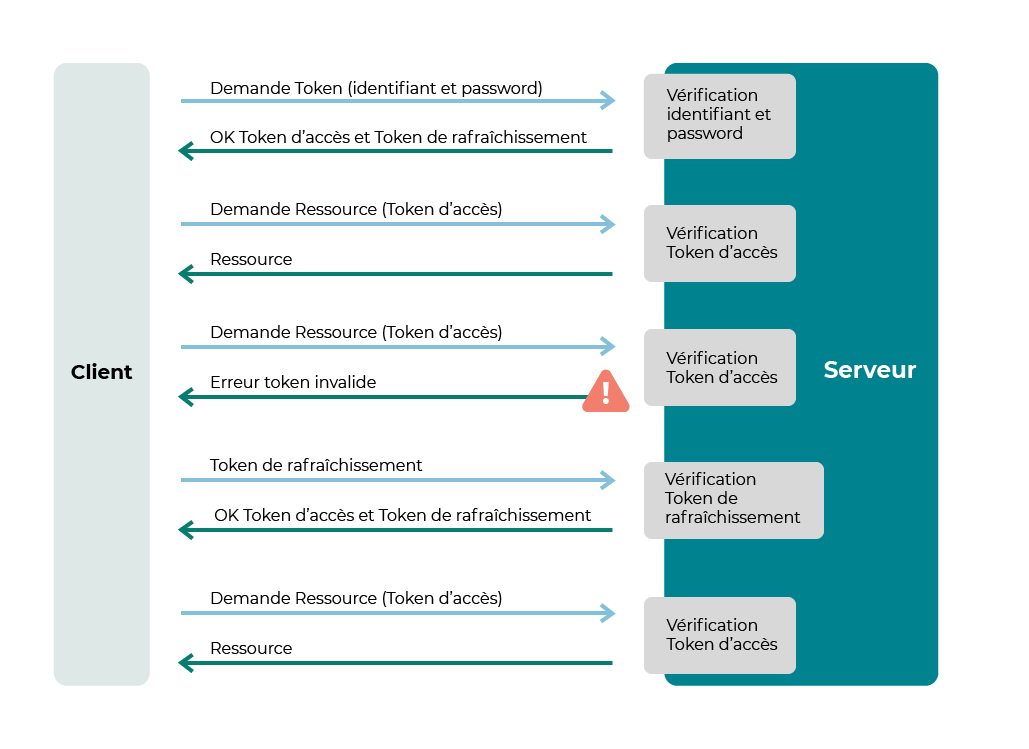
\includegraphics[width=12cm]{images/image23.png}
\end{center}
Le client envoie des demandes pour accéder aux ressources au serveur avec des tokens. Si le token est valide, le serveur envoie la ressource et un token de rafraîchissement.
Le client fournit des tokens au serveur pour accéder aux ressources

\subsection{Obtenez des tokens}
La {\color{monOrange}gestion des tokens} est un processus réalisé par les applications clientes – voyons ensemble comment fonctionne ce processus. Dans ce cours, nous allons utiliser \href{https://www.postman.com}{Postman}. Il s’agit d’un outil permettant de modifier toutes les informations de la requête qui appelle notre API. Dans le cas de {\color{monOrange}l’authentification}, nous aurons besoin entre autres de modifier les headers des requêtes.

Vous pouvez obtenir des tokens via un appel POST sur l'endpoint d’obtention de tokens que nous avons configuré dans le projet.

Un identifiant et un mot de passe doivent être fournis dans le corps de la requête, sous les noms {\tt username}  et {\tt password}. Lorsque l’authentification est en succès, alors une paire de tokens est retournée.
\begin{center}
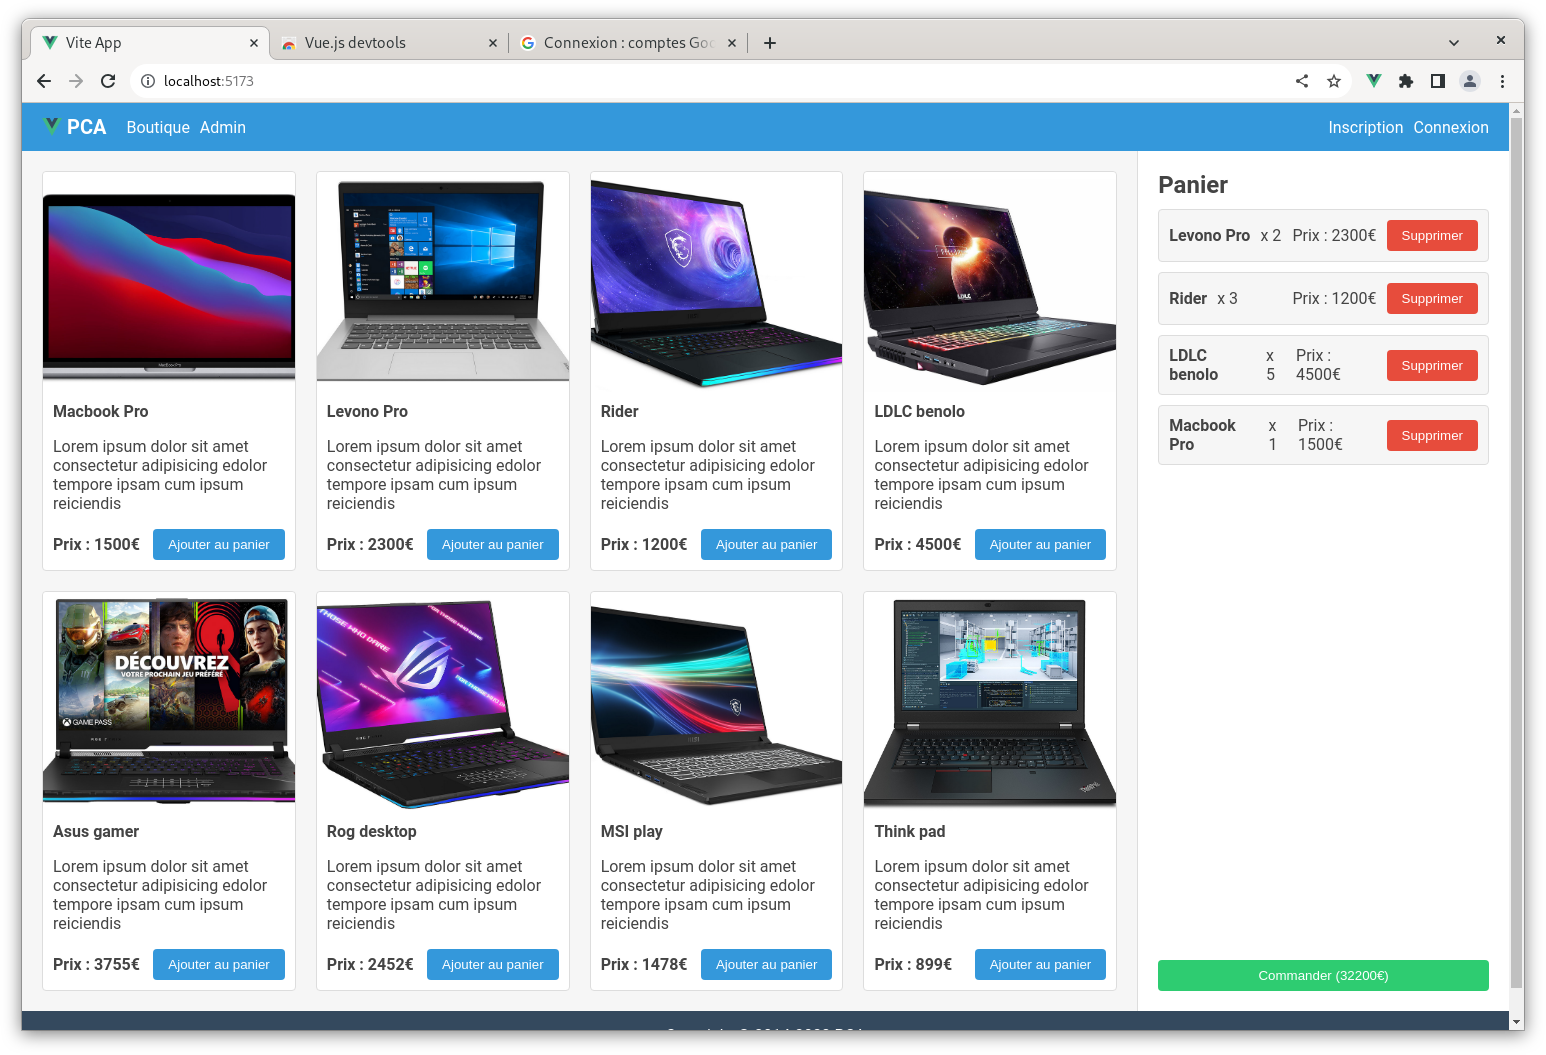
\includegraphics[width=15cm]{images/image24.png}
\end{center}
En entrant l’identifiant admin-oc et le mot de passe password-oc, nous obtenons bien deux tokens refresh et access, une paire de tokens sont retournés

\subsubsection*{C’est quoi Postman ? Pourquoi on ne reste pas dans le navigateur ?}
C’est un outil de gestion de collection d’API très utile lorsqu’on travaille en équipe, mais aussi disponible gratuitement pour un seul utilisateur. Il permet de {\color{monOrange}sauvegarder des appels API} et de réaliser plus facilement le {\color{monOrange}paramétrage de nos appels} (gestion des headers, corps de la requête, etc.).

Nous pouvons voir que chaque token est un JWT, et consiste en 3 parties séparées par des points. Chacun de ces tokens a un {\color{monOrange}rôle bien spécifique} et doit être {\color{monOrange}conservé} par l’application cliente afin de garantir la connexion de l’utilisateur.

Le token d’accès doit être transmis dans le header de chaque requête faite au serveur dans la clé nommée {\tt Authorization}. Cette clé doit avoir pour valeur  {\tt Bearer TOKEN}, en remplaçant  {\tt TOKEN}   par la valeur du token d’accès.



Dans l’onglet Headers, nous voyons la clé Authorization et le Bearer TOKEN associé
La clé Authorization et le Bearer TOKEN
\begin{center}
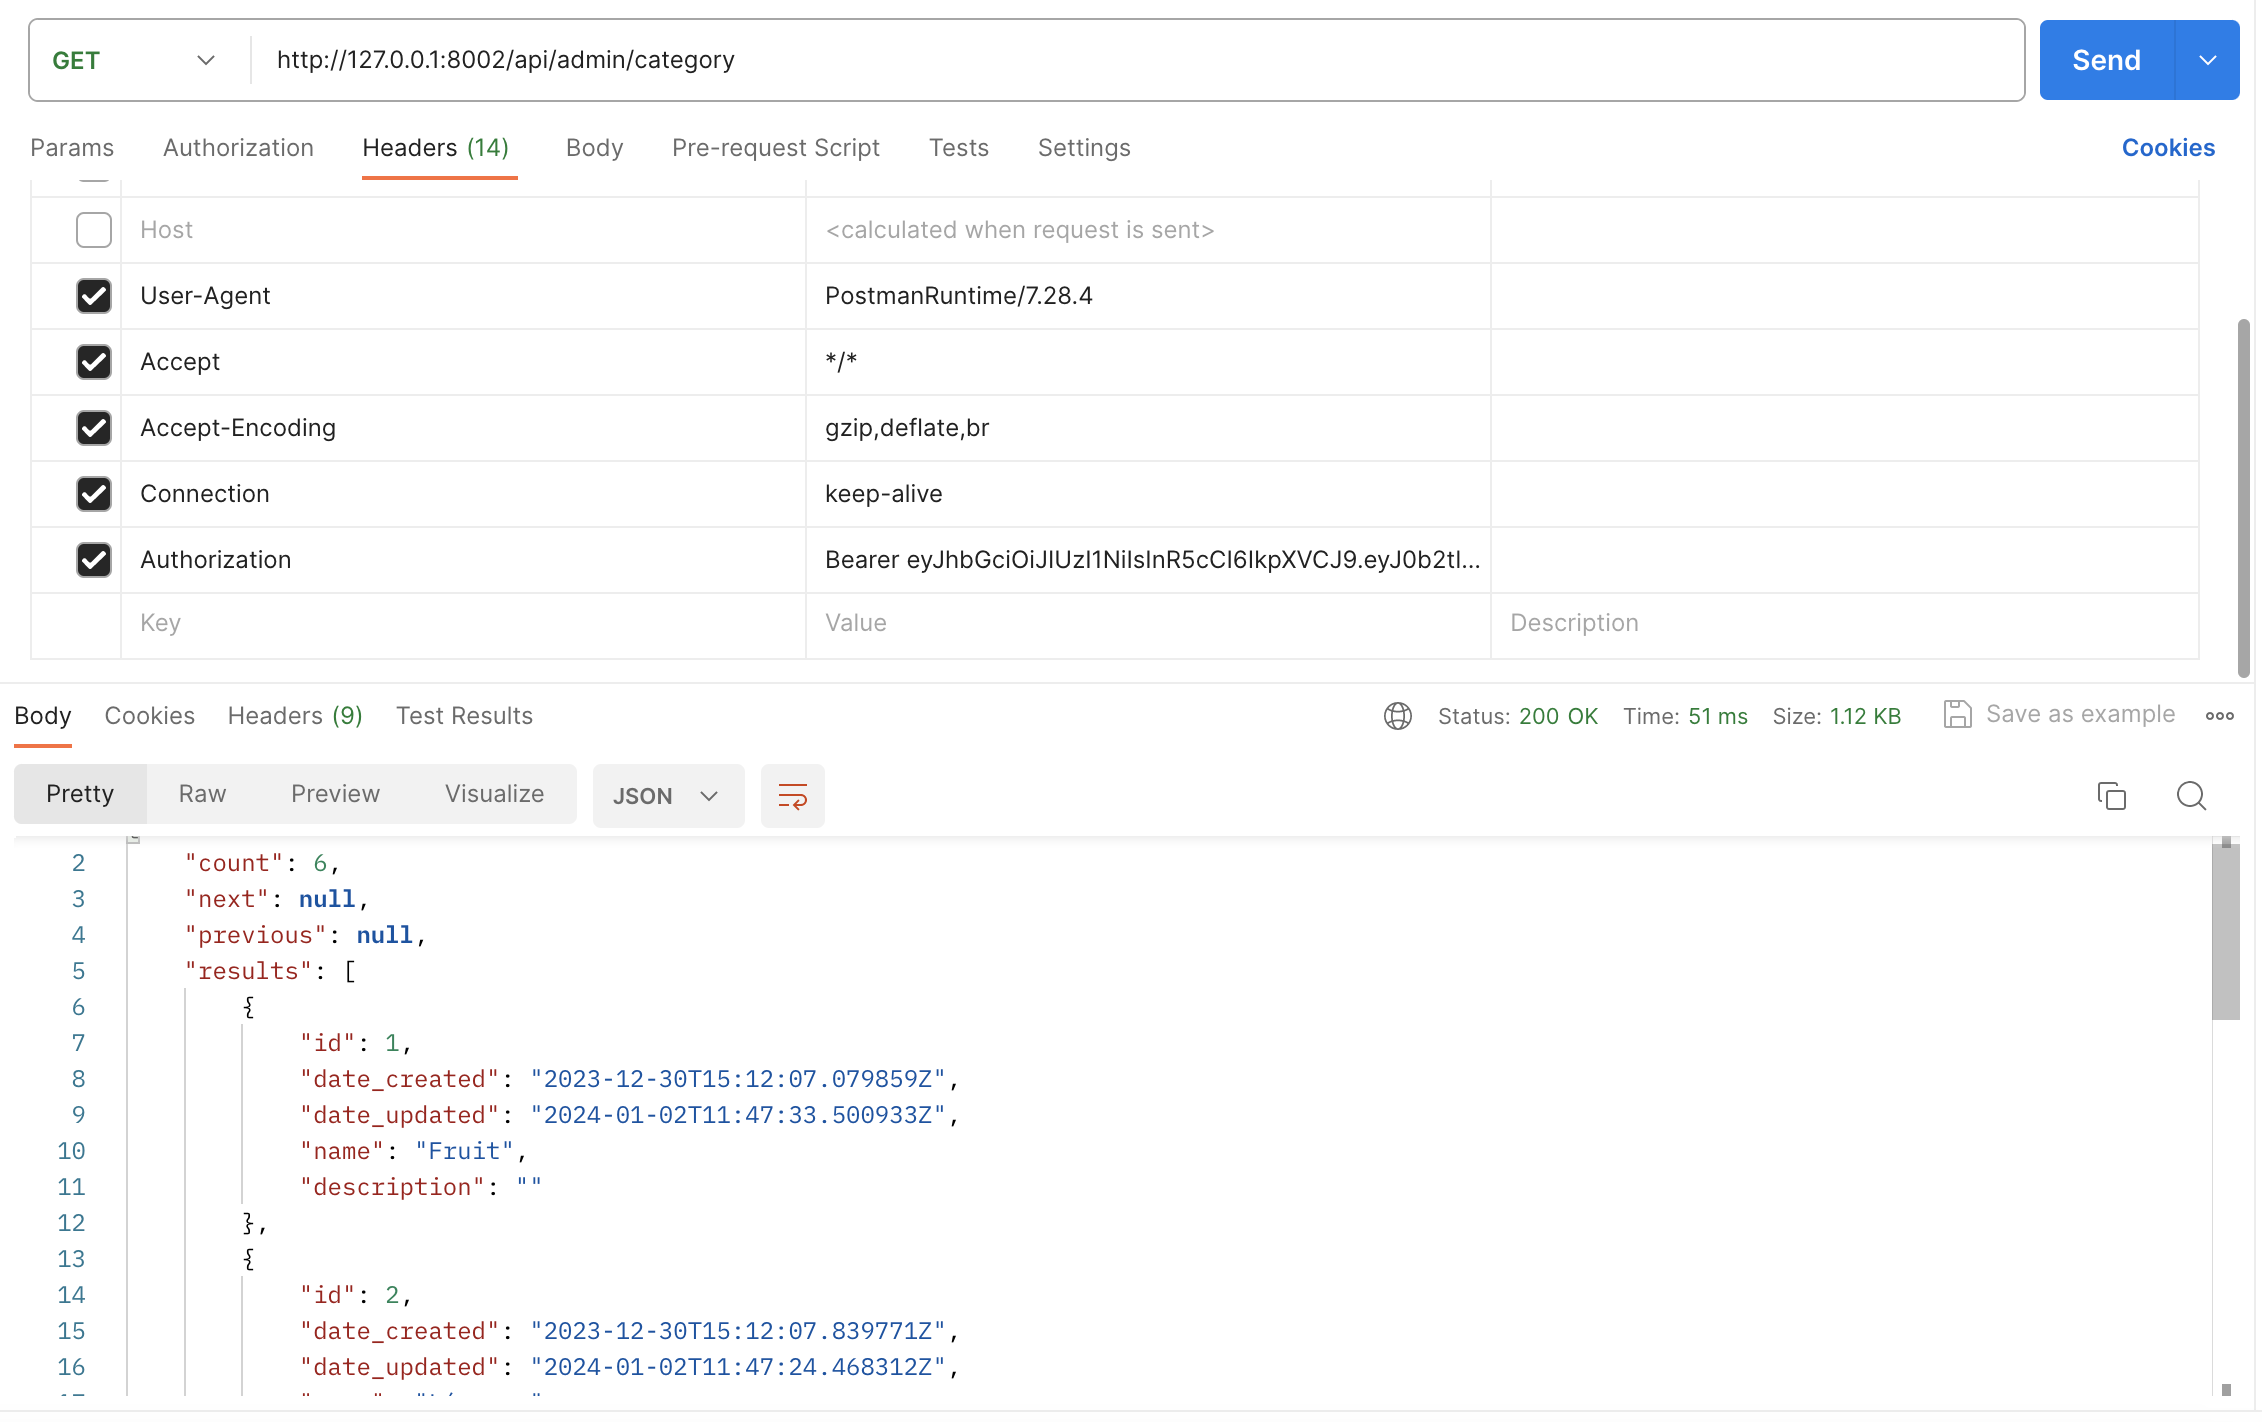
\includegraphics[width=15cm]{images/image25.png}
\end{center}

De cette façon, le serveur, en recevant la requête, peut déterminer l’utilisateur réalisant la requête.

Le token d’accès a une durée de vie {\color{monOrange}limitée dans le temps} ; si nous décodons son payload en utilisant par exemple jwt.io :
\begin{minted}[
mathescape,
framesep=2mm,
baselinestretch=1.2,
%fontsize=\footnotesize,
bgcolor=LightGray,
%linenos
]{python}
{
    "token_type": "access",
    "exp": 1628927720,
    "jti": "63e4e6dab0494aee803fed93f24a80c1",
    "user_id": 1
}
\end{minted}

... nous pouvons voir différentes informations :
\begin{itemize}
\item {\tt token\_type}  indique le type de token ;
\item {\tt exp}  est un timestamp indiquant jusqu’à quand ce token peut être utilisé ;
\item {\tt jti}  signifie JWT ID, c’est un identifiant unique créé lors de la génération du token ;
\item {\tt user\_id}  est l’identifiant Django de l’utilisateur, il est ajouté par Simple JWT lors de la génération du token.
\end{itemize}

\subsubsection*{Est-il possible de modifier la durée de vie des tokens ?}
Oui, la durée de vie des tokens peut être configurée dans les settings de Django.
\begin{minted}[
mathescape,
framesep=2mm,
baselinestretch=1.2,
%fontsize=\footnotesize,
bgcolor=LightGray,
%linenos
]{python}
SIMPLE_JWT = {
    'ACCESS_TOKEN_LIFETIME': timedelta(minutes=5),
    'REFRESH_TOKEN_LIFETIME': timedelta(days=1),
}
\end{minted}

\subsection{Rafraîchissez des tokens}
Lorsque le token d’accès n’est plus valide, il est nécessaire d’en créer un autre. C’est à cela que sert le {\color{monOrange}token de rafraîchissement}.

Il faut pour cela réaliser un appel en POST sur l’endpoint de rafraîchissement de tokens. Le token de rafraîchissement doit être transmis dans le corps de la requête sous l’attribut {\tt refresh}  , et un nouveau token d’accès est alors retourné par le serveur.
\begin{center}
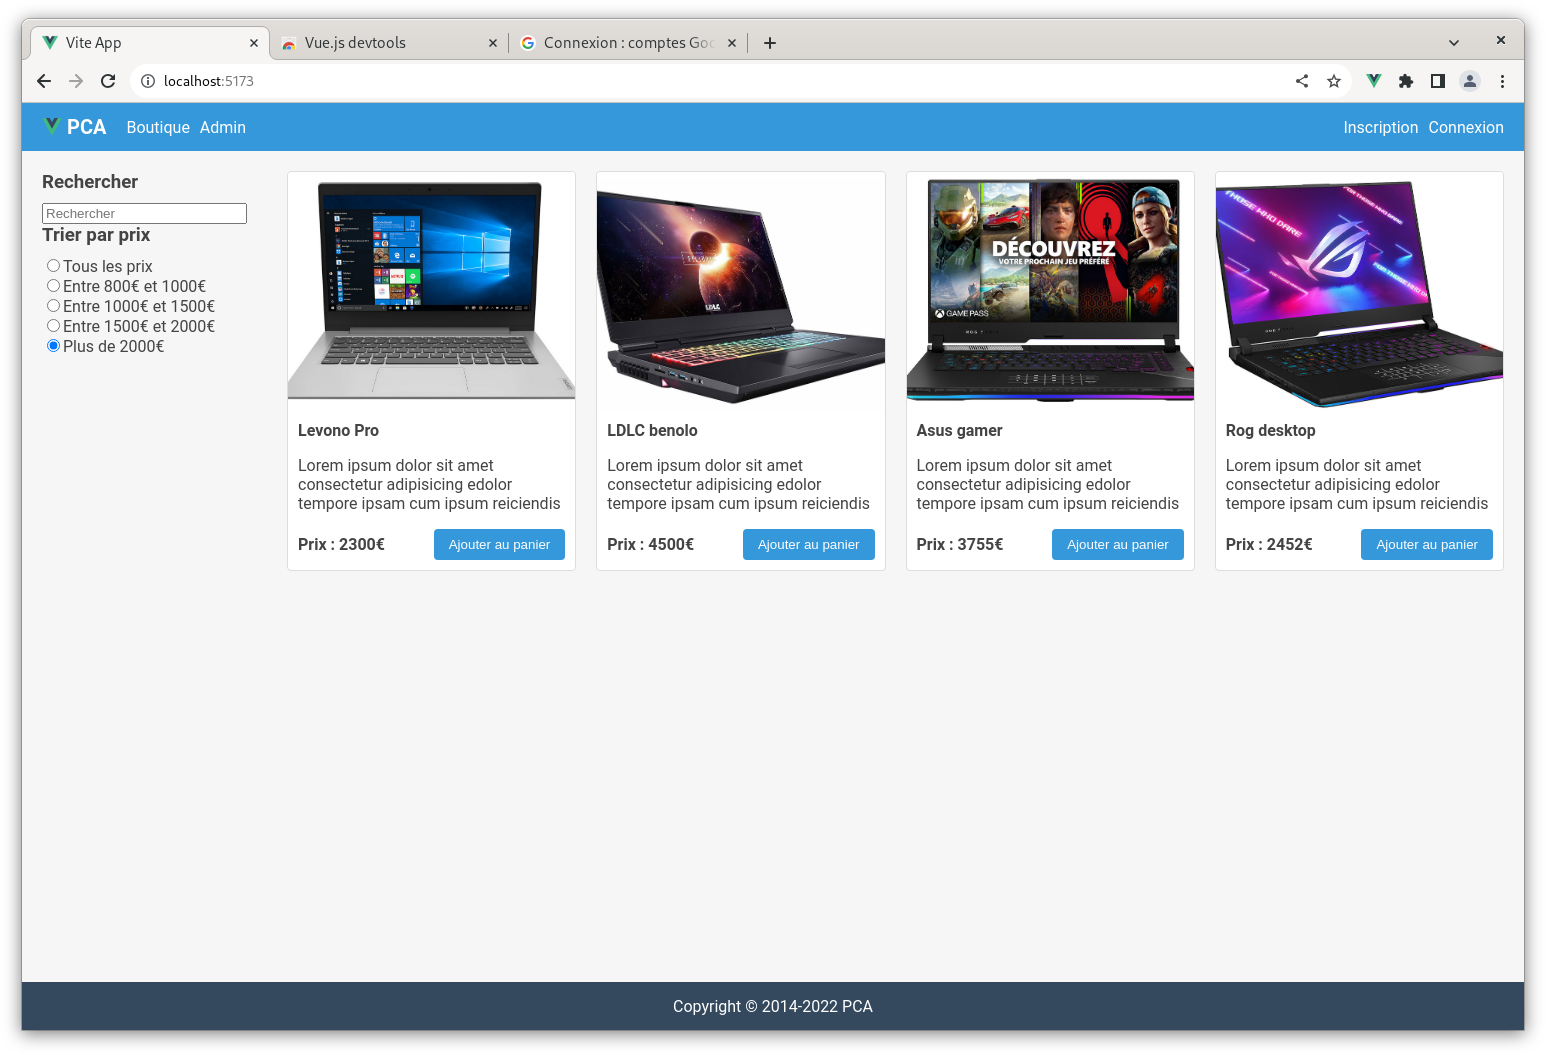
\includegraphics[width=15cm]{images/image26.png}
\end{center}
Quand nous envoyons le token de rafraîchissement, un token d’accès nous est retourné dans Postman
Le token de rafraîchissement permet d’obtenir un nouveau token d’accès
Voyons comment réaliser ces appels ensemble dans le screencast ci-dessous.


N’hésitez pas à tester le fonctionnement des tokens, comment et quand ils expirent. Chaque matin en reprenant le développement du votre projet, vos tokens devront être rafraîchis, c’est signe que l’authentification fonctionne. ;)

Le code du projet est disponible sur la branche P3C1-C2 du projet. Expérimentez la gestion des tokens comme le ferait une application cliente, afin que ce processus n’ait plus de secret pour vous !

\subsubsection*{En résumé}
\begin{enumerate}
\item Les tokens JWT sont un moyen d’assurer l’authentification des utilisateurs.
\item Les tokens d’accès et de rafraîchissement sont à conserver précieusement par les applications clientes pendant la session des utilisateurs.
\item Deux endpoints différents permettent d’une part l’obtention de tokens, et d’autre part le rafraîchissement du token d’accès.
\end{enumerate}

 {\em Maintenant que notre serveur nous permet d’obtenir et de rafraîchir des tokens, voyons dès le prochain chapitre comment limiter l’accès à certains endpoints}.
%%%%%%%%%%%%%%%%%%%%%%%%%%%%%%%%%%%%%%%%%%%%%%%%%%%%%%%%%%%%%%%%%%%%%%%%

\section{Restreignez l'accès à certains endpoints}
\subsection{Limitez l’accès aux utilisateurs authentifiés}
Nous disposons maintenant d’endpoints d’administration qui permettent de gérer pleinement des entités, mais leur accès est pour le moment {\color{monOrange}public}. Améliorons cela en imposant aux utilisateurs d’être authentifiés pour pouvoir faire des appels à nos endpoints d’administration. Commençons par l'endpoint d’{\color{monOrange}administration des catégories}.

DRF nous permet de {\color{monOrange}gérer l’accès aux endpoints} au travers des permissions, et nous propose une permission {\tt IsAuthenticated}, exactement ce qu’il nous faut !

Les permissions se configurent au niveau des views, au travers de l’attribut de classe {\tt permission\_classes}. Cet attribut est une liste, et permet donc d’appliquer plusieurs permissions. Elles sont parcourues une à une par DRF, et l’accès à la vue n’est permis que si toutes les permissions le permettent.

Mettons en place cette permission sur notre {\tt AdminCategoryViewset}  :
\begin{minted}[
mathescape,
framesep=2mm,
baselinestretch=1.2,
%fontsize=\footnotesize,
bgcolor=LightGray,
%linenos
]{python}
from rest_framework.permissions import IsAuthenticated
 
class AdminCategoryViewset(MultipleSerializerMixin, ModelViewSet):
 
    serializer_class = CategoryListSerializer
    detail_serializer_class = CategoryDetailSerializer
    # Nous avons simplement à appliquer la permission sur le viewset
    permission_classes = [IsAuthenticated]
 
    def get_queryset(self):
        return Category.objects.all()
\end{minted}

L’accès à l'endpoint nécessite à présent d’être authentifié en ajoutant dans les headers de la requête POST la clé {\tt Authorization}  qui a pour valeur  {\tt Bearer ACCESS}, où {\tt ACCESS}  est la valeur du token d’accès.

Appel en succès d’un endpoint sécurisé en précisant l’attribut Authorization dans le header de la requête
Appel en succès d’un endpoint sécurisé en précisant l’attribut Authorization dans le header de la requête
\begin{center}
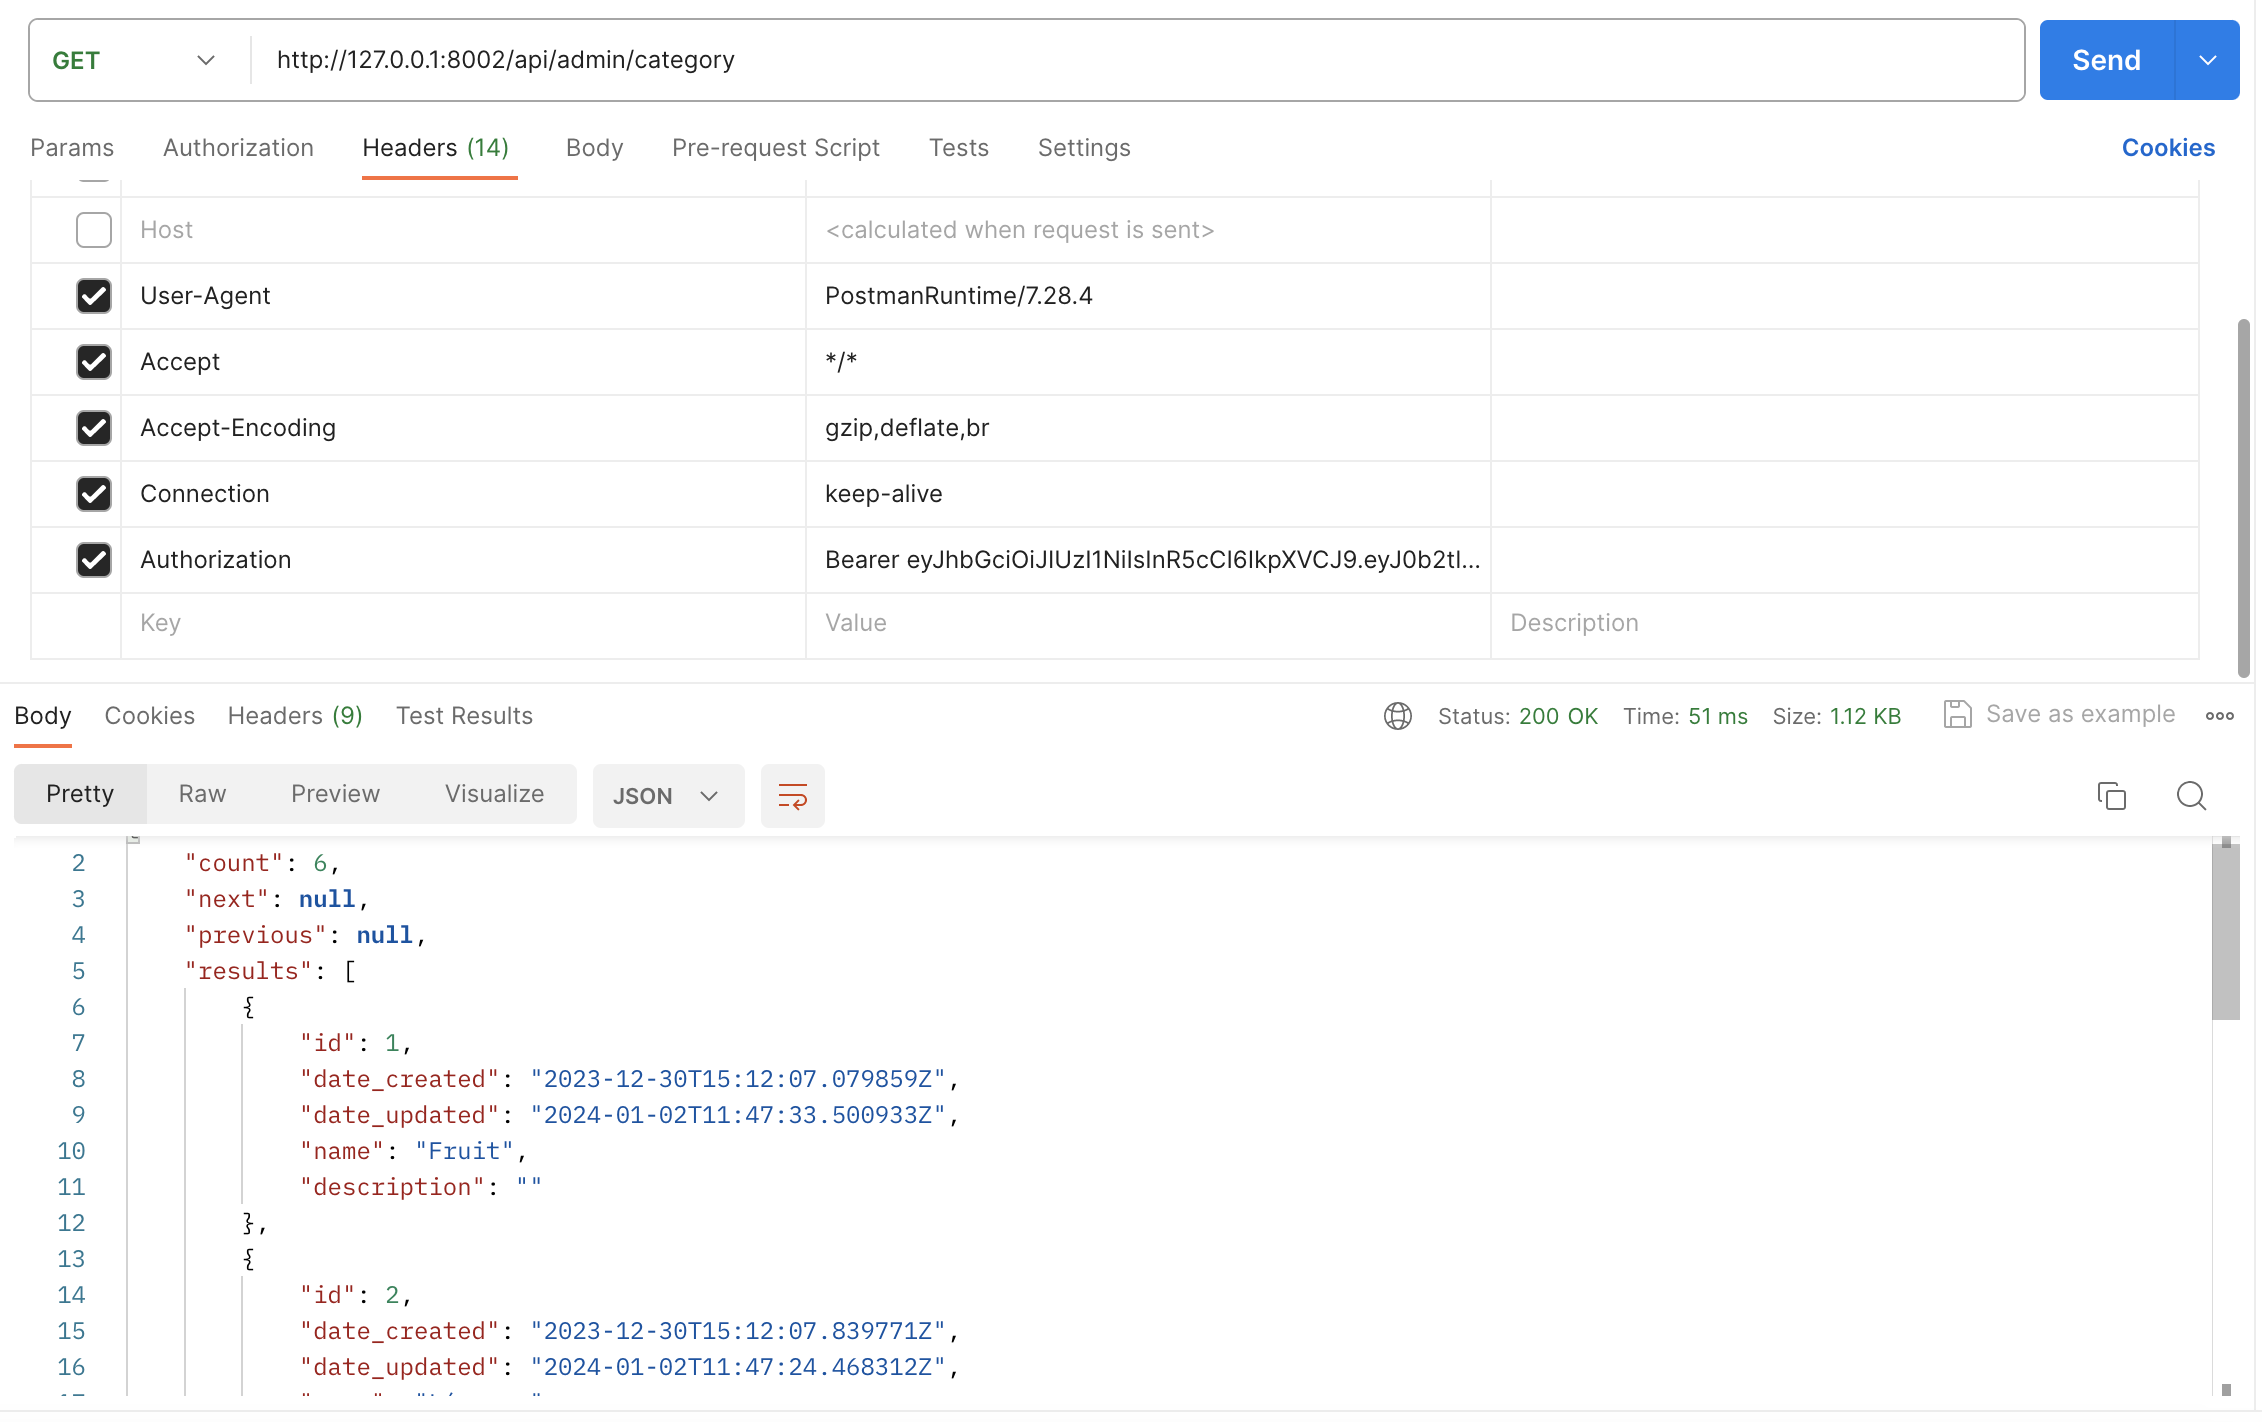
\includegraphics[width=15cm]{images/image25.png}
\end{center}

Vous verrez le status code à droite entre les KEY et la console. Ci-dessus, l'accès a été accepté et un status code 200 est retourné. Sans authentification, un status code 401 est retourné, et l’accès est {\color{monOrange}refusé}.

Un appel sans disposer d’un JWT valide ou sans en fournir sur un endpoint sécurisé retourne un status code 401


Voyons la mise en place d'authentification dans le screencast ci-dessous :

\begin{theorem}
Lors de la création d’un endpoint, il est important de penser à son accès, car il retourne peut-être des informations {\color{monOrange}confidentielles} ou permet des {\color{monOrange}actions} qui ne doivent pas être permises à tout le monde.
\end{theorem}

\subsection{Créez des permissions plus fines}
\subsubsection*{Nous venons de limiter l’accès aux personnes authentifiées, mais est-ce suffisant ?}
La réponse est non, c’est un {\color{monOrange}premier niveau de sécurité}, mais en l’état, les clients de notre boutique pourraient alors administrer nos catégories en disposant seulement d’un compte utilisateur.

DRF propose des permissions, je vous propose encore mieux ! De {\color{monOrange}créer les nôtres}. ;)

Faisons ensemble en sorte que {\color{monOrange}seuls les administrateurs} puissent accéder à cet endpoint. Créons un fichier nommé {\tt permissions.py}  dans notre application Django {\tt shop}.
\begin{minted}[
mathescape,
framesep=2mm,
baselinestretch=1.2,
%fontsize=\footnotesize,
bgcolor=LightGray,
%linenos
]{python}
from rest_framework.permissions import BasePermission
 
class IsAdminAuthenticated(BasePermission):
 
    def has_permission(self, request, view):
    # Ne donnons l’accès qu’aux utilisateurs administrateurs authentifiés
        return bool(request.user and request.user.is_authenticated and request.user.is_superuser)
\end{minted}
Il ne nous reste plus qu’à modifier notre vue pour utiliser notre nouvelle permission :
\begin{minted}[
mathescape,
framesep=2mm,
baselinestretch=1.2,
%fontsize=\footnotesize,
bgcolor=LightGray,
%linenos
]{python}
from shop.permissions import IsAdminAuthenticated
 
class AdminCategoryViewset(MultipleSerializerMixin, ModelViewSet):
 
    serializer_class = CategoryListSerializer
    detail_serializer_class = CategoryDetailSerializer
    permission_classes = [IsAdminAuthenticated]
 
    def get_queryset(self):
        return Category.objects.all()
\end{minted}
Notre endpoint est à présent {\color{monOrange}protégé} et accessible seulement aux {\color{monOrange}administrateurs authentifiés}. Un simple compte utilisateur ne suffit plus pour pouvoir y accéder.

Suivez-moi dans le screencast ci-dessous pour voir comment j'ai mis en place des permissions plus fines pour nos administrateurs :


Les permissions permettent la mise en place de règles de contrôle strictes. Avoir une permission par « acteur » (clients, partenaires, utilisateurs, administrateurs, etc.) de notre API est un bon moyen de gérer qui peut accéder à quels endpoints.

\subsubsection*{Exercice}
Allons plus loin dans nos contrôles ! Pour diverses raisons, un utilisateur administrateur n’est pas membre de l’équipe de la boutique. Il faudrait qu'il puisse n'avoir accès à l’administration qu'en tant que {\color{monOrange}prestataire}, et nous ne souhaitons pas qu’il puisse ajouter de nouvelles catégories.

Je vous propose donc de mettre en place une {\color{monOrange}nouvelle permission} qui va vérifier que l’utilisateur fasse également partie de l’équipe, en vérifiant que {\tt is\_staff}  du model {\tt User}  est bien à {\tt True}.

Les deux permissions pourront alors être mises en place sur le Viewset d’administration de catégorie.

Disposer de deux permissions nous permettra par la suite de donner l’accès à certains endpoints aux membres de l’équipe sans qu’ils aient besoin de disposer d’un compte administrateur, par exemple.

Pour réaliser cela, vous pouvez partir de la branche P2C3\_exercice. Elle contient déjà ce que nous venons de faire ensemble. Une solution est proposée sur la branche P2C3\_solution.

\subsubsection*{En résumé}
\begin{enumerate}
\item Les permissions permettent de limiter l’accès aux endpoints.
\item DRF fournit certaines permissions, mais il est possible de créer les nôtres.
\item Disposer une permission par acteur permet de facilement savoir sur quels endpoints les permissions doivent être placées.
\item Lors de la mise en place d’un nouvel endpoint, il est important de savoir qui va l’utiliser, pour déterminer s’il doit rester public ou doit posséder certaines permissions.
\end{enumerate}
{\em Notre API est toute sécurisée. Je vous invite maintenant à valider vos acquis de cette partie dans le quiz. Après, nous reviendrons sur tout ce que vous avez accompli pendant ce cours !}




%\end{document}










